\documentclass[usenames,dvipsnames,10pt,pdf,utf8,russian,aspectratio=43]{beamer}
\usepackage[english,russian]{babel}
\usepackage{cmap}
\usepackage[T2A]{fontenc}
\usepackage{subfig}
\usepackage{color}
\usepackage{tikz}
%\usepackage{tikz,fullpage}
\DeclareMathOperator*{\argmax}{arg\,max}
\DeclareMathOperator*{\argmin}{arg\,min}

\usetikzlibrary{arrows,automata}
\usetikzlibrary{positioning}

%
% Choose how your presentation looks.
%
% For more themes, color themes and font themes, see:
% http://deic.uab.es/~iblanes/beamer_gallery/index_by_theme.html
%


\mode<presentation>
{


  \usetheme{Boadilla}      % or try Darmstadt, Madrid, Warsaw, ...
  \usecolortheme{seagull} % or try albatross, beaver, crane, ..

 \usefonttheme{structurebold}  % or try serif, structurebold, ...
  \setbeamertemplate{navigation symbols}{}
  \setbeamertemplate{caption}[numbered]
} 


\captionsetup[subfloat]{labelformat=empty}
\title[Выбор структуры]{Выбор структуры модели глубокого обучения}
\author{Бахтеев Олег}
\institute{МФТИ}
\date{13.02.2019}

\begin{document}

\begin{frame}
  \titlepage
\end{frame}


\begin{frame}{Графовое представление модели глубокого обучения}
\begin{block}{Определение}
Задан  граф $(V,E)$. Для каждого ребра $(j,k) \in E$ определен вектор базовых функций  мощности $K^{j,k}$: $$\mathbf{g}^{j,k} = [\mathbf{g}^{j,k}_0, \dots, \mathbf{g}^{j,k}_{K^{j,k}}]$$. Пусть для каждой вершины $v \in V$ определена функция агрегации $\textbf{agg}_v$.\\ Граф $(V, E)$ в совокупности со множестом векторов базовых функций $\{\mathbf{g}^{j,k}, (j,k) \in E\}$ и множеством функций агрегаций $\{ \textbf{agg}_v, {v \in V}\}$ называется \textit{параметрическим семейством моделей} $\mathfrak{F}$, если функция, задаваемая как 
\begin{equation}
\label{eq:modelfam}
    \mathbf{f}_k(\mathbf{x}) = \textbf{agg}_k\left(\{ \langle \boldsymbol{\gamma}^{j,k}, \mathbf{g}^{j,k} \rangle \left(\mathbf{f}_j(\mathbf{x})\right)| j \in \text{Adj}(v_k)\}\right), \quad \mathbf{f}_0(\mathbf{x}) = \mathbf{x}
\end{equation}
является моделью при любых значениях векторов, $\boldsymbol{\gamma}^{j,k} \in [0,1]^{K^{j,k}}$.

\end{block}
\end{frame}

\begin{frame}{Пример: двуслойная нейросеть}
\begin{figure}
\small
\begin{tikzpicture}[node distance=cm, auto]
  %\tikzstyle{every state}=[fill=red,draw=none,text=white]

  \node (f0)  at (1,6)                  {$\mathbf{f}_0(\mathbf{x}) = \mathbf{x}$};
  %\node (g11) at (6,3)                    {$\mathbf{g}^{1,1}(\mathbf{x})$};% = \text{Conv}(\mathbf{x}, 3, 32, 1)$};
  %\node (g12)  at (6,9)                   {$\mathbf{g}^{1,2}(\mathbf{x})$};% = \text{Conv}(\mathbf{x}, 4, 32, 1)$};
  \node (f1)  at (5,6)                 {$\mathbf{f}_1(\mathbf{x})$};% = \gamma^{1,1}\mathbf{g}^{1,1}(\mathbf{x}) +  \gamma^{1,2}\mathbf{g}^{1,2}(\mathbf{x})$};
  %\node (g21) at (12,6)                   {$\mathbf{g}^{2,1}(\mathbf{x})$};% = \boldsymbol{\sigma}(\mathbf{w}^{2,1}\mathbf{x})$};
  \node (f2)  at (10,6)                   {$\mathbf{f}_2(\mathbf{x})$};% = \gamma^{2,1}\mathbf{g}^{2,1}(\mathbf{x})$};
  \path[->]  (f0) edge [bend left=50] node {$\mathbf{g}^{0,1}_0(\mathbf{x}) = \boldsymbol{\sigma}(\mathbf{w}^{0,1}_0\mathbf{x})$}(f1);
  \path[->] (f0)  edge[bend right=50] node[below] {$\mathbf{g}^{0,1}_1(\mathbf{x}) = \boldsymbol{\sigma}(\mathbf{w}^{0,1}_1\mathbf{x})$}(f1);
  \path[->] (f1)  edge node {$\mathbf{g}^{1,2}_0(\mathbf{x}) = \textbf{softmax}(\mathbf{w}^{1,2}_0\mathbf{x})$}(f2);       
  \draw[->] (f1) to (f2);
 
\end{tikzpicture}

\end{figure}
\end{frame}

\begin{frame}{Пример: сверточная сеть}
\small
\begin{figure}
\begin{tikzpicture}[node distance=0.5cm, auto]
  %\tikzstyle{every state}=[fill=red,draw=none,text=white]

  \node (f0)  at (1,6)                  {$\mathbf{f}_0(\mathbf{x}) = \mathbf{x}$};
  %\node (g11) at (6,3)                    {$\mathbf{g}^{1,1}(\mathbf{x})$};% = \text{Conv}(\mathbf{x}, 3, 32, 1)$};
  %\node (g12)  at (6,9)                   {$\mathbf{g}^{1,2}(\mathbf{x})$};% = \text{Conv}(\mathbf{x}, 4, 32, 1)$};
  \node (f1)  at (5,6)                 {$\mathbf{f}_1(\mathbf{x})$};% = \gamma^{1,1}\mathbf{g}^{1,1}(\mathbf{x}) +  \gamma^{1,2}\mathbf{g}^{1,2}(\mathbf{x})$};
  %\node (g21) at (12,6)                   {$\mathbf{g}^{2,1}(\mathbf{x})$};% = \boldsymbol{\sigma}(\mathbf{w}^{2,1}\mathbf{x})$};
  \node (f2)  at (10,6)                   {$\mathbf{f}_2(\mathbf{x})$};% = \gamma^{2,1}\mathbf{g}^{2,1}(\mathbf{x})$};
  \path[->]  (f0) edge [bend left=50] node {$\mathbf{g}^{0,1}_0(\mathbf{x}) = \textbf{Conv}(\mathbf{x}, c_0, c_1)$}(f1);
  \path[->] (f0)  edge[bend right=50] node[below] {$\mathbf{g}^{0,1}_1(\mathbf{x}) = \textbf{Conv}(\mathbf{x}, 1, c_1) \circ \textbf{Conv}(\mathbf{x}, c_0, c_2)$}(f1);
  \path[->] (f1)  edge node {$\mathbf{g}^{1,2}_0(\mathbf{x}) = \textbf{softmax}(\mathbf{w}^{2,1}\mathbf{x})$}(f2);            
  \draw[->] (f1) to (f2);
 
\end{tikzpicture}

\end{figure}
\end{frame}



\begin{frame}{Ограничения на структурные параметры}
\begin{figure}
  \centering
{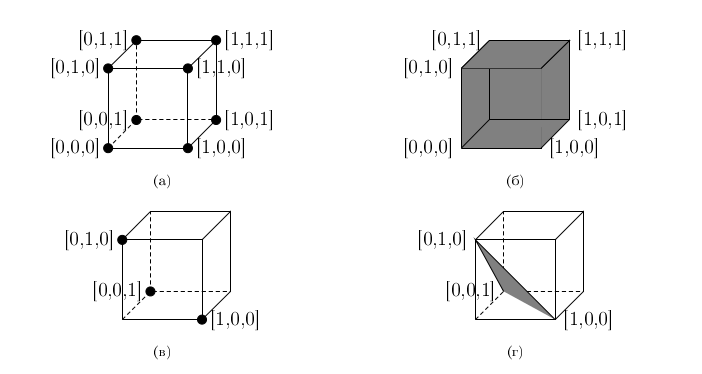
\includegraphics[width=0.8\textwidth]{cubes.png}} 
\end{figure}

\end{frame}





\begin{frame}{Статистические критерии качества модели}


\textbf{Параметрическая сложность} --- наименьшая дивергенция между априорным распределением параметров и апостериорным распределением параметров:
\[
    C_\text{param} = \min_{\mathbf{h}} \text{D}_\text{KL}(p(\mathbf{W}, \boldsymbol{\Gamma}|\mathbf{y}, \mathbf{X})||p(\mathbf{W}, \boldsymbol{\Gamma}||\mathbf{h})).
\]



\textbf{Структурная сложность модели} --- энтропия апостериорного распределения структуры модели:
\[
    C_\text{struct} = -\mathsf{E}_{p} \text{log}~p(\boldsymbol{\Gamma}|\mathbf{y}, \mathbf{X}).
\]

\end{frame}


\begin{frame}{Выбор оптимальной модели}
\textbf{Основные проблемы выбора оптимальной модели}\\
\begin{itemize}
\item Интеграл правдоподобия $p(\mathbf{y}|\mathbf{X}, \mathbf{h})$ невычислим аналитически.
\item Задача его оптимизации многоэкстремальна и невыпукла.
\end{itemize}
~\\
\textbf{Требуется}\\ 
Предложить метод поиска субоптимального решения задачи оптимизации, обобщающего различные алгоритмы оптимизации:
\begin{itemize}
\item Оптимизация правдоподобия.
\item Последовательное увеличение и снижение сложности модели.
\item Полный перебор вариантов структуры модели.
\end{itemize}

\end{frame} 
   


\begin{frame}{ Распределение на структуре}
Пусть для каждого ребра $(j,k)$ задан нормированный положительный вектор $\boldsymbol{\gamma}_{j,k} \in \mathbb{R}_{+}^{|K_{j,k}|}$, определяющий веса базовых функций из  $\mathbf{g}(j,k)$. Перечислим основные свойства, которыми должно обладать распределение такого вектора:
\begin{enumerate}
\item $p(\boldsymbol{\gamma}^{j,k})$ является непрерывным на симплексе $\Delta^{K^{j,k}-1}$.
\item При устремлении температуры к бесконечности распределение сходится к равномерному: $\lim_{c_{\text{temp}} \to \infty} = p(\boldsymbol{\gamma}^{j,k})| \text{c}_{\text{temp}}) = \mathcal{U}(\Delta^{K^{j,k}-1}).$
\item При устремлении температуры к нулю распределение сходится к сингулярному распределению следующего вида:
$$\lim_{c_{\text{temp}} \to 0}  p(\gamma^{j,k}_k) = m^{j,k}_k,$$ где $\mathbf{m}^{j,k}$ --- параметр распределения.
\end{enumerate}


\end{frame}


\begin{frame}{Варианты распределений}
\begin{enumerate}
\item Дирихле;
\item Гумбель-Софтмакс: 
\[
    \hat{\boldsymbol{\gamma}}_h = \text{exp}\left(\text{log}\left(m_h + \text{Gum}_h\right)c_{\text{temp}}^{-1}\right) \sum_{l=1}^{K_{j,k}} \text{exp}\left(\text{log}\left(m_l + \text{Gum}_l\right)c_{\text{temp}}^{-1}\right),
\]
где $\text{Gum} \sim -\text{log}(-\text{log}~\mathcal{U}(0,1)).$ 
\end{enumerate}

\begin{figure}
  \centering
{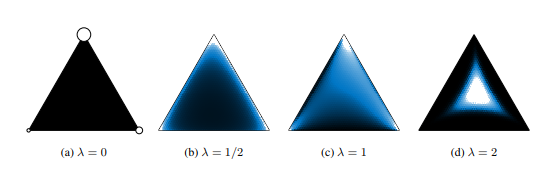
\includegraphics[width=0.8\textwidth]{gs.png}} 
\end{figure}

Maddison et al., 2017.
\end{frame}



\begin{frame}{Оптимизация параметров вариационного распределения}

Параметры вариационного распределения $q(\mathbf{W}, \boldsymbol{\Gamma}) = q_{\mathbf{W}}(\mathbf{W})q_{\boldsymbol{\Gamma}}(\boldsymbol{\Gamma})$ оптимизируем:
\[
L =
\textcolor{blue}{\mathsf{E}_q \text{log}~{p(\mathbf{y} | \mathbf{X}, \mathbf{W}, \boldsymbol{\Gamma}. \mathbf{A}^{-1}, c_{\text{temp}})}} -$$ $$- \textcolor{red}{c_\text{reg}\text{D}_{KL}\left(p(\mathbf{w}, \boldsymbol{\Gamma} |\mathbf{A}^{-1}, \mathbf{m}, c_{\text{temp}}) || q(\mathbf{W}), q(\boldsymbol{\Gamma})\right)} \to \max_{\mathbf{A}_q, \boldsymbol{\mu}_q, \mathbf{m}_q}.
\]

\begin{block}{Теорема}
Пусть $c_\text{reg} > 0$ .
Тогда $\frac{1}{m}L(c_\text{reg})$ сходится п.н. к той же функции, что и $\frac{c_\text{reg}}{m_0}L(c_\text{reg}=1)$.
\end{block}
\textbf{Интерпретация: } для достаточно большого $m$ и $c_\text{reg} \neq 1$ оптимизация параметров и гиперпараметров эквивалентна оптимизации ELBO для выборки другой мощности.
\end{frame}
\begin{frame}

\begin{block}{Теорема  [Бахтеев, 2018].}
Пусть $\boldsymbol{\Gamma}_1$ и $\boldsymbol{\Gamma}_2$ --- реализации $\boldsymbol{\Gamma}$, такие что:
\begin{itemize}
\item $\boldsymbol{\Gamma}_1 \in \bar{\Delta}(\boldsymbol{\Gamma})$.
\item $\boldsymbol{\Gamma}_2 \not \in \bar{\Delta}(\boldsymbol{\Gamma})$.
\end{itemize} 
Тогда для любых положительно определенных матриц $\mathbf{A}_1$ и $\mathbf{A}_2$ и векторов $\mathbf{m}_1, \mathbf{m}_2, \text{min}(\mathbf{m}_1)>0$ справедлива следующее отношение апостериорных вероятностей:
$$\lim_{c_\text{temp} \to 0} \frac{p(\boldsymbol{\Gamma}_2, \mathbf{W}_2|\mathbf{y},  \mathbf{X},\mathbf{A}_1,\mathbf{m}_2, {c_\text{temp}})}{p(\boldsymbol{\Gamma}_1,  \mathbf{W}|\mathbf{y}, \mathbf{X},\mathbf{A}_1,\mathbf{m}_1, {c_\text{temp}})} = \infty.$$
\end{block}
\end{frame}


\begin{frame}{Оптимизация параметров априорного распределения}
\small
Гиперпараметры $\mathbf{A}, \mathbf{m}$ оптимизируем:
\[
Q = \textcolor{blue}{c_\text{train}\mathsf{E}_q \text{log}~{p(\mathbf{y} | \mathbf{X}, \mathbf{W}, \boldsymbol{\Gamma}. \mathbf{A}^{-1}, c_{\text{prior}})}}
 - \textcolor{red}{c_\text{prior}\text{D}_{KL}(p(\mathbf{W}, \boldsymbol{\Gamma} |\mathbf{A}^{-1}, \mathbf{m}, c_{\text{temp}}) || q(\mathbf{W}, \boldsymbol{\Gamma}))} -\]
\[
 - \textcolor{OliveGreen}{c_{\text{comb}}\sum_{p' \in \mathbf{P}} \text{D}_{KL}(\boldsymbol{\Gamma} | p')} \to \max, 
\]
где $\mathbf{P}$ --- множество (возможно пустое) распределений на структуре модели.
\begin{itemize}
\item $\textcolor{blue}{c_\text{train}}$ --- коэффициент правдоподобия выборки;
\item $\textcolor{red}{c_\text{prior}}$ --- коэффициент регуляризации модели;
\item $\textcolor{OliveGreen}{c_{\text{comb}}}$ --- коэффициент перебора структуры.
\end{itemize}
\end{frame}

\begin{frame}{Общая задача оптимизации}
\small
Общая задача оптимизации --- двухуровневая:
\[
\hat{\mathbf{A}}, \hat{\mathbf{m}} = \argmax_{\mathbf{A}, \mathbf{m}} Q = 
\]
\[
= \textcolor{blue}{c_\text{train}\mathsf{E}_{\hat{q}} \text{log}~{p(\mathbf{y} | \mathbf{X}, \mathbf{W}, \boldsymbol{\Gamma}. \mathbf{A}^{-1}, c_{\text{prior}})}}
 - \textcolor{red}{c_\text{prior}\text{D}_{KL}(p(\mathbf{W}, \boldsymbol{\Gamma} |\mathbf{A}^{-1}, \mathbf{m}, c_{\text{temp}}) || \hat{q}(\mathbf{W}, \boldsymbol{\Gamma}))} -\]
\[
 - \textcolor{OliveGreen}{c_{\text{comb}}\sum_{p' \in \mathbf{P}} \text{D}_{KL}(\boldsymbol{\Gamma} | p')}, 
\]
где 
\[
\hat{q} = \argmax_{q} L = 
\textcolor{blue}{\mathsf{E}_q \text{log}~{p(\mathbf{y} | \mathbf{X}, \mathbf{W}, \boldsymbol{\Gamma}. \mathbf{A}^{-1}, c_{\text{temp}})}} - \textcolor{red}{c_\text{reg}\text{D}_{KL}(p(\mathbf{w}, \boldsymbol{\Gamma} |\mathbf{A}^{-1}, \mathbf{m}, c_{\text{temp}}) || q(\mathbf{W}), q(\boldsymbol{\Gamma}))}
\]

\end{frame}





\begin{frame}{Параметрическая сложность}
Обозначим за $F(c_{\text{reg}}, c_{\text{train}}, c_{\text{prior}}, c_{\text{comb}}, \mathbf{P}, c_{\text{temp}})$ множество экстремумов функции $L$ при решении задачи двухуровневой оптимизации.
\begin{block}{Утверждение}
Пусть $\mathbf{f} \in F(1, 1, c_{\text{prior}}, 0, \varnothing,  c_{\text{temp}} )$.
При устремлении $ c_{\text{prior}}$ к бесконечности параметрическая сложность модели $\mathbf{f}$ устремляется к нулю.
\[
    \lim_{c_{\text{prior}} \to \infty} C_{\text{param}}(\mathbf{f}) = 0.
\]
\end{block}
\end{frame}

\begin{frame}{Параметрическая сложность}
Обозначим за $F(c_{\text{reg}}, c_{\text{train}}, c_{\text{prior}}, c_{\text{comb}}, \mathbf{P}, c_{\text{temp}})$ множество экстремумов функции $L$ при решении задачи двухуровневой оптимизации.
\begin{block}{Утверждение}
Пусть $\mathbf{f}_1 \in F(1, 1, c_{\text{prior}}^1, 0, \varnothing,  c_{\text{temp}} ), \mathbf{h}_2 \in F(1, 1, c_{\text{prior}}^2, 0, \varnothing,  c_{\text{temp}})$, $c_{\text{prior}}^1 < c_{\text{prior}}^2$.\\
Пусть вариационные параметры моделей $\mathbf{f}_1$ и $\mathbf{f}_2$ лежат в области $\mathsf{U}$, в которой соответствующие функции $L$ и $Q$ являются локально-выпуклыми.\\ 
Тогда модель $\mathbf{f}_1$ имеет параметрическую сложность, не меньшую чем у $\mathbf{f}_2$.
\[
    C_\text{param}(\mathbf{f}_1) \geq C_\text{param}(\mathbf{f}_2).
\]
\end{block}


\end{frame}

\begin{frame}{Структурная сложность}

\begin{block}{Утверждение}
Пусть для каждого ребра $(i,j)$ семейства моделей $\mathfrak{F}$ априорное распределение $$p(\boldsymbol{\gamma}_{i,j}) =  \lim_{c_{\text{temp}} \to 0} \mathcal{GS}(c_{\text{temp}}).$$
Пусть $c_{\text{reg}} >0, c_{\text{train}} >0, c_{\text{prior}}>0$.
Пусть $\mathbf{f} \in F(c_{\text{reg}}, c_{\text{train}}, c_{\text{prior}}, 0, \varnothing, c_{\text{temp}})$.
Тогда структурная сложность модели $\mathbf{f}$ равняется нулю.
\[
    C_\text{struct}(\mathbf{f}) = 0.
\]
\end{block}
\end{frame}

\begin{frame}{Структурная сложность}
\begin{block}{Гипотеза}
Пусть $\mathbf{f}_1 \in F(c_{\text{reg}}, c_{\text{train}},  c_{\text{prior}}, 0, \varnothing,  c^1_{\text{temp}}), \mathbf{h}_2   \in \lim_{c^2_{\text{temp}} \to \infty} F(c_{\text{reg}}, c_{\text{train}},  c_{\text{prior}}, 0, \varnothing,  c^2_{\text{temp}})$.
Пусть вариационные параметры моделей $f_1$ и $f_2$ лежат в области $U$, в которой соответствующие функции $L$ и $Q$ являются локально-выпуклыми. 
Тогда разница структурных сложностей моделей ограничена выражением:
\[
    C_\text{struct}(\mathbf{f}_1)  - C_\text{struct}(\mathbf{f}_2) \leq \textcolor{blue}{\mathsf{E}_q^1 \text{log}~{p(\mathbf{y} | \mathbf{X}, \mathbf{W}, \boldsymbol{\Gamma}. \mathbf{A}^{-1}, c^1_{\text{temp}})}} - \textcolor{blue}{\mathsf{E}_q^2 \text{log}~{p(\mathbf{y} | \mathbf{X}, \mathbf{W}, \boldsymbol{\Gamma}, \mathbf{A}^{-1})}}.
\]
\end{block}

% Схема доказательства:
% расписываем неравенства вида: L_1 - DKL(q_1|p1) <L_2 - DKL(q_2|p1)
% Замечаем, что при стремлении к бесконечности гумбель превращается в равномерное
% выражаем все в равномерном
% замечаем, что D_KL = Entropy + const для равномерного
% все
\end{frame}


\begin{frame}{Полный перебор}
\small
Пусть для каждого ребра $(i,j)$ семейства моделей $\mathfrak{F}$ априорное распределение $$p(\boldsymbol{\gamma}_{i,j}) =  lim_{c_{\text{temp}} \to 0} \mathcal{GS}(c_{\text{temp}}).$$

Рассмотрим последовательность $\mathbf{P}$, состоящую из $N = \prod_{(j,k) \in E} K_{j,k}$ моделей, полученных в ходе оптимизаций вида:
$$f_1 \in F(c_{\text{reg}}, 0, 0, \varnothing, c_{\text{comb}},  c_{\text{temp}}),$$
$$f_2 \in F(c_{\text{reg}}, 0, 0, \{q_1(\boldsymbol{\Gamma})\},  c_{\text{comb}},  c_{\text{temp}}),$$
$$f_3 \in F(c_{\text{reg}}, 0, 0, \{q_1(\boldsymbol{\Gamma}), q_2(\boldsymbol{\Gamma})\},  c_{\text{comb}},  c_{\text{temp}}),$$
где $C_{\text{reg}} > 0,  c_{\text{comb}}>0$.


\begin{block}{Гипотеза}
Вариационные распределения $q_{\boldsymbol{\Gamma}}$ структур  последовательности $\mathbf{P}$ вырождаются в распределения вида $\delta(\hat{\mathbf{m}})$, где $\hat{\mathbf{m}}$ --- точка на декартовом произведении вершин симплексов структуры модели.

Последовательность соответствует полному перебору структуры $\boldsymbol{\Gamma}$.
\end{block}
\end{frame}

\end{document}

